\documentclass[10pt,twocolumn,letterpaper]{article}

\usepackage{cvpr}
\usepackage{times}
\usepackage{epsfig}
\usepackage{graphicx}
\usepackage{amsmath}
\usepackage{amssymb}
\usepackage{CJKutf8}
% Include other packages here, before hyperref.

% If you comment hyperref and then uncomment it, you should delete
% egpaper.aux before re-running latex.  (Or just hit 'q' on the first latex
% run, let it finish, and you should be clear).
\usepackage[breaklinks=true,bookmarks=false]{hyperref}

\cvprfinalcopy % *** Uncomment this line for the final submission

\def\cvprPaperID{****} % *** Enter the CVPR Paper ID here
\def\httilde{\mbox{\tt\raisebox{-.5ex}{\symbol{126}}}}

% Pages are numbered in submission mode, and unnumbered in camera-ready
%\ifcvprfinal\pagestyle{empty}\fi
\setcounter{page}{1}
\begin{document}
\begin{CJK}{UTF8}{bsmi}

%%%%%%%%% TITLE
\title{Auto Turn Sheet Music}

\author{林郁翔\\
P76094509\\
{\tt\small richardlin0212@gmail.com}
% For a paper whose authors are all at the same institution,
% omit the following lines up until the closing ``}''.
% Additional authors and addresses can be added with ``\and'',
% just like the second author.
% To save space, use either the email address or home page, not both
\and
方嘉祥\\
P76094151\\
{\tt\small frank870622@gmail.com}
}

\maketitle
%\thispagestyle{empty}

%%%%%%%%% ABSTRACT
\begin{abstract}
   For a song you played for the first time, you usually need to look at the sheet music to play, and most pile of sheet music are not only one page, so you must turn page when you are about to finish playing the page.

   We want to develop a software that can automatically scroll the guitar tablature with the progress of the music according to the input music or video.
\end{abstract}

%%%%%%%%% BODY TEXT
\section{Introduction}

Anyone who has experience in playing musical instruments knows that most musical instruments require both hands to play.
Most pile of sheet music have more than one page, so when you are about to finish one page, you must turn a page.
For paper-made sheet music, you can line up the papers without turning pages, but if you want to see all the sheet music on electronic scores, you must reduce the sheet music to a small size, and notes are too small to see.

When practicing guitar, if it is not a self-created piece or a covered song, it is usually played with the existing music, usually a popular music film. If you only list the chords, most of them don’t need to turn pages, but the guitar tabs that pay more attention to fingering are usually presented in the form of six-line tabs, tablatures, corresponding to the first to sixth strings of the guitar from top to bottom. Tablature may present in many aspects. It can come with five-line staff(Figure ~\ref{fig:tab1}), or show alone(Figure ~\ref{fig:tab2}). At this time, the number of tablature pages will rise quickly, and the number of times the sheet music will be flipped will also increase significantly. At this time, if you are practicing against existing music, you will interrupt the practice when you turn the page, or you want to focus on practicing a certain paragraph, you need to turn the sheet music to the position at the same time, and the music must be fixed to a certain place, which is a waste of time .

\begin{figure}[t]
\begin{center}
   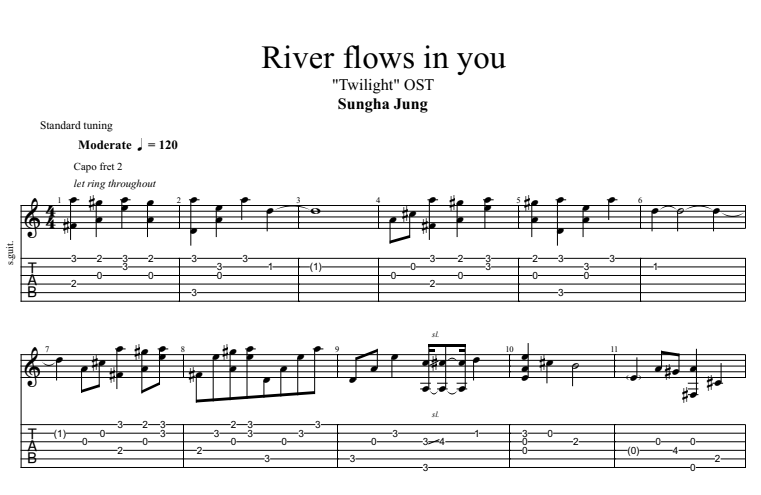
\includegraphics[width=0.9\linewidth]{tablature.png}
\end{center}
\caption{Example of Guitar Tabs with staff\cite{river_flows_in_you}}
\label{fig:long}
\label{fig:tab1}
\end{figure}

\begin{figure}[t]
\begin{center}
   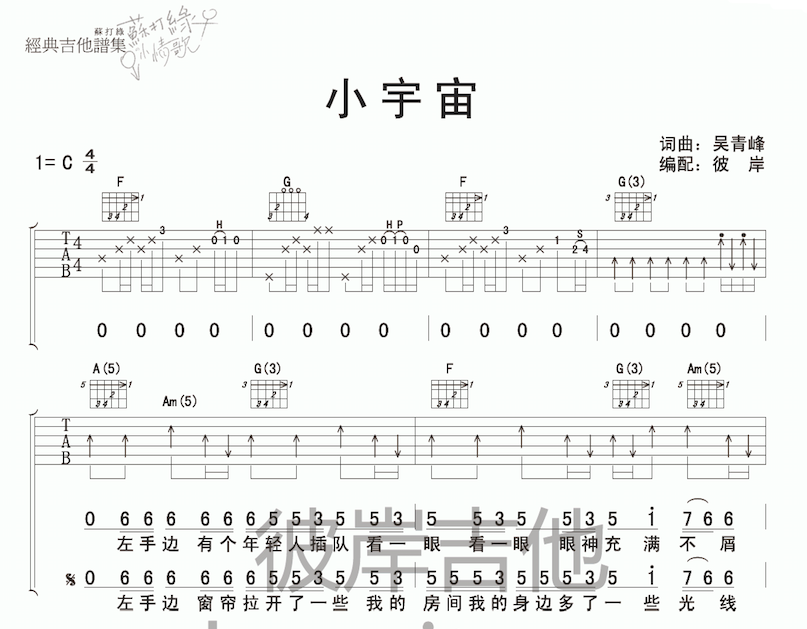
\includegraphics[width=0.9\linewidth]{tab2.png}
\end{center}
\caption{Example of Guitar Tabs without staff\cite{small_universe}}
\label{fig:long}
\label{fig:tab2}
\end{figure}

We want to develop a software that can automatically scroll the tablature with the progress of the music according to the input guitar music or video, and in conjunction with the input tablature. Existing software requires a certain format (gp5, midi) to perform related work. We want to analyze the most common pdf and scroll the tablatures stored in the pdf according to the music. We also hope that users can pause the music at any time, or adjust the music to an appropriate position, and the tablature will also reach the correct paragraph.

%------------------------------------------------------------------------
\section{System framework}

\begin{figure*}
\begin{center}
    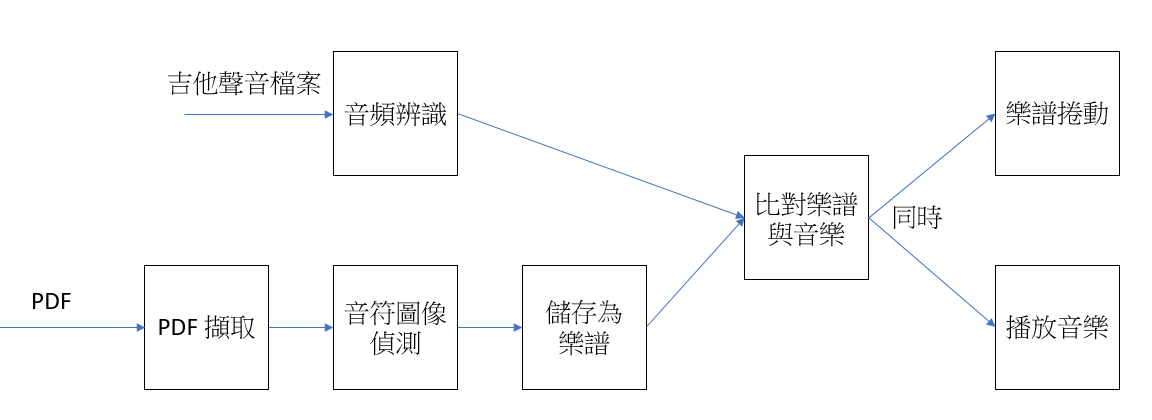
\includegraphics[width=1\linewidth]{step1.png}
\end{center}
   \caption{System framework.}
\label{fig:step1}
\end{figure*}
We will read the tablature in PDF format and record them as gp5 format. When inputting music later, we can automatically detect the beat and pitch, find out the position of the current tablatures, and then scroll the tablature with the music(Figure ~\ref{fig:step1}). 


%------------------------------------------------------------------------
\section{Expected results}

We hope to do like Tonara\cite{Tonara}, which scrolls staff automatically.(Figure ~\ref{fig:tonara}) We also want our application to play music according to the current cursor on the tablature. When the user pauses or moves the cursor of the tablature, our application will play the music according to it. Just like what Guitar Pro\cite{GuitarPro} can do.(Figure ~\ref{fig:gp75})

\begin{figure}[t]
\begin{center}
   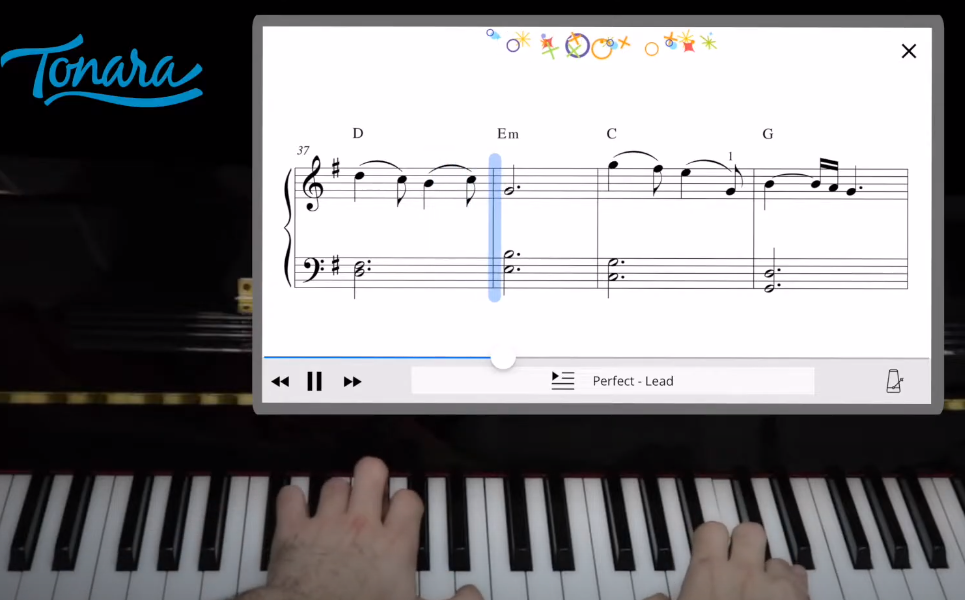
\includegraphics[width=0.8\linewidth]{tonara.png}
\end{center}
   \caption{Example of Tonara\cite{Tonara2}}
\label{fig:long}
\label{fig:tonara}
\end{figure}

\begin{figure}[t]
\begin{center}
   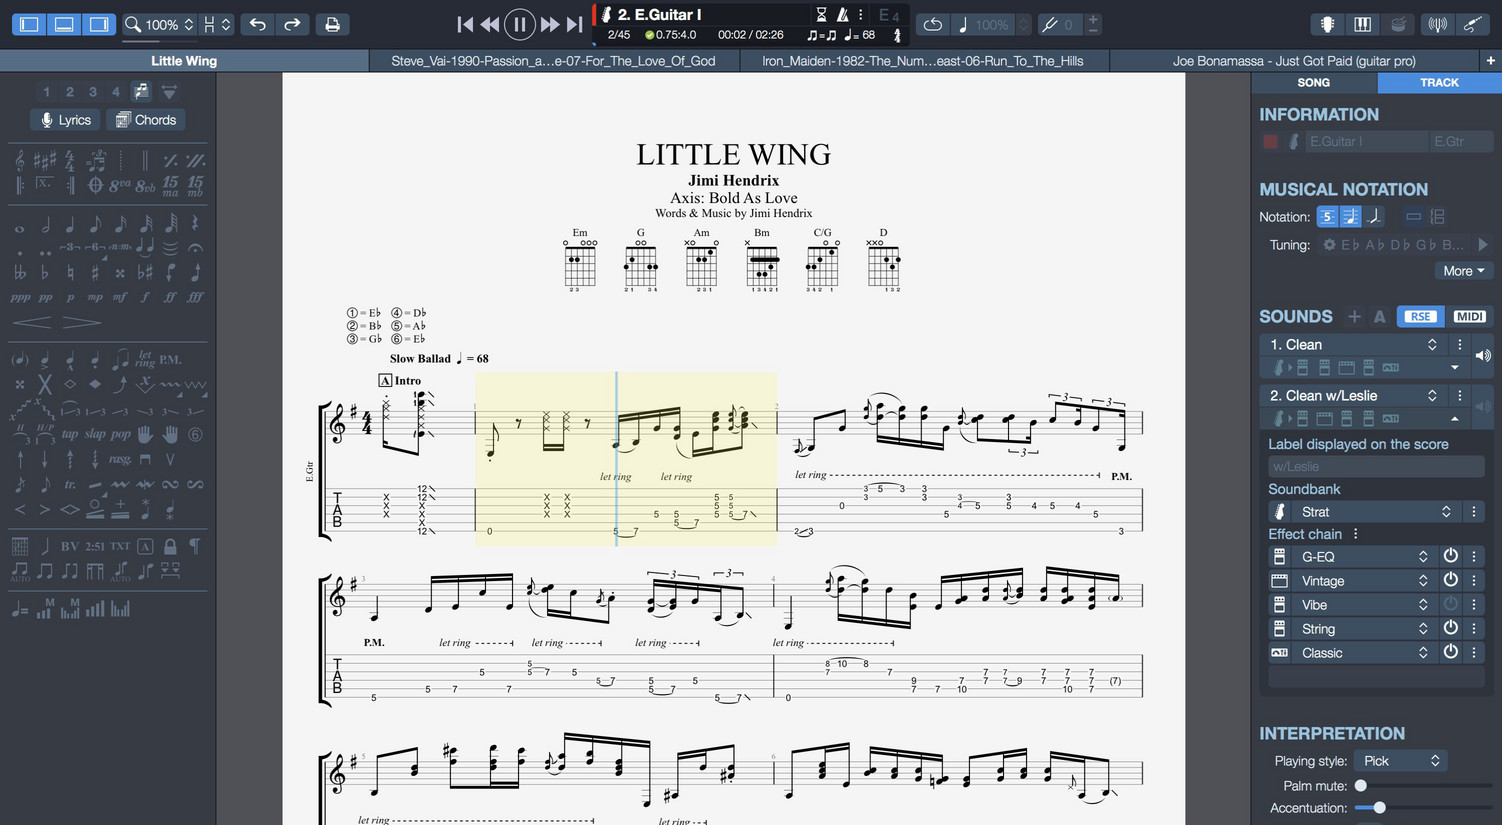
\includegraphics[width=0.8\linewidth]{gp75.jpg}
\end{center}
   \caption{Example of Guitar Pro\cite{GuitarPro}}
\label{fig:long}
\label{fig:gp75}
\end{figure}


{\small
\bibliographystyle{ieee_fullname}
\bibliography{egbib}
}

\end{CJK}
\end{document}
